Most, hogy már túl vagyunk a konténerek mibenlétének megtárgyalásán, ideje azzal foglalkozni milyen \textit{widget}eket lehet a konténerekben elhelyezni. Az első és talán legkézenfekvőbb megoldás erre a kérdésre egy beviteli mező, hiszen ablakaink jelentékeny részét arra ahsználjuk, hogy a felhasználótól adatokat kérjünk be. Ez a rész az beviteli mezőkkkel általános és az egysoros bevitelő mezők konkrét fejlesztési és tesztelési kérdéseivel foglalkozik.

\section{Fogalmak}

\subsection{Beviteli mezők típusai}

Az adatbevitelre szolgáló \textit{widget}ek számos szempont szerint csoportosíthatóak. Ezek közül csak a legkézenfekvőbbeket vesszük röviden sorra, azokat addig a mértékig, amíg ezen rész szempontjából érdekesek.

\subsubsection{Bevitt adat típusa szerint}

Gyakorlatilag minden adat bevihető szövegként, ugyanakkor nem mindig ez a leginkább célravezető módszer. Felhasználó szempontból egy üresen álló szöveges beviteli mező meglehetősen kétségbeejtő látvány. Ilyen esetben ugyanis semmi nem utal arra, hogy voltaképpen a beviteli mezőt milyen milyen típusú, formátumú, hosszú, kódolású lehet feltölteni. Emiatt mindig célszerű a lehető legspecifikusabb \textit{widget}et alkalmazni. Emellett persze az is igaz, hogy a leggyakoribb beviteli eszközünk mégiscsak a szöveges beviteli mező marad.

\includetwingraphics
{Szövegbeviteli mező\cite{gtkref}}
{entry}
{entry.png}
{Számbeviteli mező\cite{gtkref}}
{spinbutton}
{spinbutton.png}
{Szöveg és szám bevitele}
{widgetinheritance}


\paragraph{Szöveg}

A szöveg bevitele tehát a legáltalánosabb szükséglet, amit egy \textit{UI} kapcsán elképzelni lehet, mégis számos olyan funkció létezik, ami egy szöveges bevitelt lehetővé tevő \textit{widget}nek teljesítenie kell. Ilyen például kijelölés, a másolás, a beillesztés, beszúrás, a unicode karakterek kezelése, a használt betűtípus-paraméterek megadásának lehetősége akár karakterenként. Erre a \textit{GTK} szöveges bevitelre alkalmas \textit{widget}ei természetesen mind képesek, sőt, de erről majd később.

\paragraph{Szám}

Számok bevitele gyakorlatilag a szövegbevitel egyfajta specializációja, legalábbis a bevitel ellenőrzésének tekintetében. Számok bevitele esetén nyilván csak számjegyeket, illetve a számok beviteléhez kapcsolódó egyéb karaktereket (tizedes vessző, előjel, \dots), engedünk bevinni. Emellett egy widget ezen kívül nyújthat még egyéb kényelmi szolgáltatásokat is amik megkönnyítik a fejlesztők munkáját, min például a minimális, maximális elfogadható érték, tizedes jegyek számának meghatározása, lépésköz megadása az érték lépésenkénti megváltoztatásához, vagy akár számként való beállítás, illetve lekérdezés lehetősége.

\subsubsection{Sorok száma szerint}

A sorok száma szerint mindössze két típus megkülönböztetésének van létjogosultsága. Az egy, illetve a több sor kezelésére alkalmas \textit{widget}ek mind a felhasználás körében, mind a kezelés módjában, mind pedig a tesztelésben gyökeresen eltérnek egymástól.

\paragraph{Egysoros beviteli mezők}

Ezen beviteli mezők esetén a tárolt, illetve megjelenített értéket jellemzően egy egységként kezeljük. Egyszerű, néhány tíz karakternyi, adatot kérünk be ezen \textit{widget}ek segítségével, így sem különösebb szövegszerkesztési, sem pedig látványos megjelenítési funkciókat nem kell a \textit{widget}nek ellátnia. Ennek megfelelően sem a használat, sem pedig a tesztelés nem jelent alapesetben különös kihívást.

\paragraph{Többsoros beviteli mezők}

Lévén ezek a \textit{widget}ek gyakorlatilag egy egyszerűbb szövegszerkesztő alkalmazásként is felfoghatóak, akár komplett fájltartalmak kezelésére is alkalmasak, akár olyan extra funkciókkal igénybevétele mellett, mint a tartalomnak formátuménak megfelelő szintaxis kiemelés (\textit{syntax highlight}). Ennek megfelelően a kezelés sem annyira kézenfekvő, mint az egysoros \textit{widget} esetén. Tesztelési szempontból azonban -- mindaddig amíg csak a tartalmat egyben akarjuk kiolvasni, vagy beírni -- nem lesz igazán nehéz dolgunk.

\subsection{Interfész}

\index{GtkEditable@\texttt{GtkEditable}}
Azon \textit{widget}ek kezeléséhez, melyek valamilyen tartalom szerkesztésére szolgálnak -- függetlenül attól, hogy ez a tartalom szám vagy akár szöveg, egy vagy több sort foglal el -- a \textit{GTK} egy interfészt (\texttt{GtkEditable}) definiál. Ez az interfész meghatároz számos olyan műveletet (\texttt{insert\_text}, \texttt{select\_text}, \texttt{get\_position}, \dots), illetve szignált (\texttt{changed}, \texttt{delete-text}, \texttt{insert-text}), amiket az interfész megvalósító \textit{widget}nek implementálnia kell. Ennek eredményeként ezen \textit{widget}ek egy egységes felületen (\textit{API}) keresztül kezelhetőek és csak a specifikumok tekintetében kell az interfészt implementáló \textit{widget}hez tartozó függvényt, szignált használnunk.

\section{Alapműveletek}

\subsection{Létrehozás}

A létrehozás formai elemei a korábbi részek ismeretében nem okozhatnak meglepetést, így a tartalmi elemekre koncentrálunk. Mindkét \textit{widget} esetében van mire.

\subsubsection{\texttt{GtkEntry}}
\index{GtkEntry@\texttt{GtkEntry}!függvények!new@\texttt{new}}
\index{GtkEntry@\texttt{GtkEntry}!függvények!new\_with\_buffer@\texttt{new\_with\_buffer}}

A \texttt{GtkEntry} osztály esetében létezik egy paraméter nélküli konstruktor függvény (\texttt{new}), ami voltaképpen semmit különöset nem tesz. Létrehoz egy olyan \texttt{GtkEntry} objektumot, ami a tulajdonságinak alapértelmezett értékeit veszi fel, ami pontosan megfelel a hétköznapi használat szükségleteinek. A másik konstruktor függvény egy \texttt{GtkEntryBuffer} objektumot vesz át paraméterként, aminek segítségével lehetővé válik a buffer által tárolt adat megjelenítése több különböző \texttt{GtkEntry} példányban.

\index{GtkEntryBuffer@\texttt{GtkEntryBuffer}}
A \texttt{GtkEntryBuffer} voltaképpen az egysoros beviteli mező adattárolója, az ehhez szükséges kevés számú tulajdonsággal (\texttt{text}, \texttt{length}, \texttt{max-length}) és szignállal (\texttt{deleted-text}, \texttt{inserted-text}), valamint az ezen tulajdonságok beállítására, lekérdezésére -- a szokásos nevezéktan szerint --, illetve a szignálok kiváltására szolgáló függvényekkel.

\subsubsection{\texttt{GtkSpinButton}}

A \texttt{GtkSpinButton}, bár a \texttt{GtkEntry} osztályból származik, annak specializációja, attól mégis jelentékeny mértékben eltér, mind a létrehozás, mind a későbbi kezelés tekintetében. Létrehozására egy három paraméteres függvény szolgál, aminek minden paramétere szorul némi magyarázatra.

\begin{description}

 \item[adjustment] A \texttt{GtkAdjustment} egy olyan valós számot reprezentál, ami nem csupán egy magában álló érték -- hiszen erre megfelelne egy egyszerű \texttt{gdouble} is --, hanem bizonyos paraméterekkel van összerendelve. Ezek a paraméterek, a konstruktor függvénynek való átadás sorrendjében, a következők.

 \begin{description}
  \item[value] A konkrét érték.
  \item[lower, upper] Az érték által felvehető minimális, maximális érték.
  \item[step increment, page increment] Az érték falhasználó által történő növelésekor, csökkentése során használandó lépésköz. Konkrétan a \textit{le}, \textit{fel}, valamint a \textit{page down}, \textit{page up} billentyűk lenyomásakor a \texttt{step increment}, illetve a \textit{page increment} értékével csökken, illetve nő az érték. A \textit{widget} maga is tartalmaz egy fel le nyíl párost, ami az érték növelésére, csökkentésere szolgál és szintén a \texttt{step increment} értéket használja.
  \item[page size] A \texttt{GtkSpinButton} esetében nem használt beállítás.
 \end{description}

 \item[digits] A \textit{widget} által az érték megjelenítésekor használt tizedes jegyek száma.
 \item[climb rate] Az érték felhasználó általi ismétlődő növelésekor, csökkentésekor bizonyos lépésszám után használandó gyorsítási arány. Gyakorlatban a folyamatosan lenyomott \textit{le}, \textit{fel}, \textit{page down}, \textit{page up} billentyűk, illetve a \textit{widget} fel le nyilai hatására lép életben ez a mechanizmus.
\end{description}

\subsection{Tartalom kezelése}
\index{GtkEntry@\texttt{GtkEntry}!függvények!get\_text@\texttt{get\_text}}
\index{GtkEntry@\texttt{GtkEntry}!függvények!set\_text@\texttt{set\_text}}
\index{GtkEntry@\texttt{GtkEntry}!tulajdonságok!text@\texttt{text}}
\index{GtkSpinButton@\texttt{GtkSpinButton}!tulajdonságok!value@\texttt{value}}

A tartalom kezelése alapvetően kétféleképp történhet; szöveg szerint, illetve érték szerint. Természetesen a \texttt{GtkEntry} esetén csak a szöveg elérés lehetséges, míg a \texttt{GtkSpinButton} esetén mindkét mód elérhető, lévén a \texttt{GtkSpinButton} voltaképpen \texttt{GtkEntry}. A függvények nevei értelemszerűen \texttt{GtkEntry} esetén \texttt{get\_text}, illetve \texttt{set\_text}, a \texttt{get\_value}, \texttt{set\_value}, illetve \texttt{get\_value\_as\_int}, \texttt{set\_value\_as\_int}.

\subsection{Csak olvasható mód}
\index{GtkEditable@\texttt{GtkEditable}!függvények!set\_editable@\texttt{set\_editable}}

Egy alapvetően adatok bekérésére szolgáló \textit{widget} esetén a szerkeszthetőség tiltása ugyan ritka, de nem szokatlan művelet. Ennek lehetőségét a korábban már említett -- a \texttt{GtkEntry} és \texttt{GtkSpinButton} által is implementált -- \texttt{GtkEditable} interfész biztosítja. Értelemszerűen a \texttt{set\_editable} függvény az, amit hívva a szerkeszthetőséget állíthatjuk.

\subsection{Jelszavak kezelése}
\index{GtkEntry@\texttt{GtkEntry}!függvények!set\_visible@\texttt{set\_visible}}
\index{GtkEntry@\texttt{GtkEntry}!tulajdonságok!visibility@\texttt{visibility}}
\index{GtkEntry@\texttt{GtkEntry}!függvények!set\_invisible\_char@\texttt{set\_invisible\_char}}
\index{GtkEntry@\texttt{GtkEntry}!tulajdonságok!invisible-char@\texttt{invisible-char}}

A jelszavak kezelésének szempontjából két függvényt, illetve az általuk módosított tulajdonságot kell megismernünk. Az első tulajdonság \texttt{visibility}, ami alapértelmezetten \texttt{TRUE} értéket vesz fel --, meghatározza, hogy a beviteli mezőben, az annak értékül adott szöveget fogjuk látni, vagy ehelyett az azzal megegyező számú egyforma karakter. Utóbbi esetben ez a karakter, a másik megemlítendő tulajdonság (\texttt{invisible-char}) révén adható meg. Ennek alapértelmezett értékét a \textit{GTK} határozza meg a rendszeren elérhető betűkészleteknek megfelelően.

\subsection{Szignálok}

A szignálok tekintetében általában csupán a beviteli mező tartalmának változása az, ami az érdeklődésünkre számot tart. Ez a változás ugyanakkor többféle változás is lehet. Egyrészről szövegesszerű változás egy szöveges beviteli mező esetén, az érték változása szám bevitelére szolgáló \textit{widget} esetén. Ez utóbbi esetben megkülönböztethetőek azok az esetek, amikor a szöveg váltaztatása vezettett az érték változásához, illetve az az eset, amikor a \textit{widget} saját funkcióit (fel/le nyíl, page up/down billenyűk, \dots) kihasználva növeljük, illetve csökkentjük az értéket.

\subsubsection{Szöveg változása}

A \texttt{GtkEditable} típus -- ezzel együtt tehát az interfészt implementáló \texttt{GtkEntry}, illetve az abból származó \texttt{GtkSpinButton} -- \texttt{changed} szigmálja minden esetben kiváltódik, amikor a beviteli mező tartalma megvűltozik, pontosabban megváltozott. A szignált kezelő függvény már csak azt követkően hívódik meg, mután a szöveg már megvűltozott, vagyis a szignálkezelő függványben lekérdéezve már az új értéket kapjuk.

Mivel a szignál voltaképpen minden billentyű leütést -- legyen az beírás vagy törlés -- meghívódik célszerű a kezelőfüggvényben implementáltak kapcsán ezt figyelembe venni, például a lefutás időigényét a lehetőség szerinti minimumon tartani. Még ha a kód lefutása gyors is, attól érdemes óvakodni, hogy minden egyes billentyű lenyomására végrehajtsuk azt a műveletet (validáció, más felületi elemek változtatása, \dots), amit elegendő akkor megtennünk, ha a beviteli mező elvesztette a fókuszt. Az erre alkalmas szignál is adott (\texttt{focus-out}), a bevitt adatokra vonatkozó validáció (pl: IP cím, reguláris kifejezés), vagy éppen a tartalom egyéb \textit{widget}ekre gyakorolt hatásának szabályainak célszerűen amúgy sem a magából a hatásból kell kiderülniük. Erre alkalmas eszköz inkább valamely súgó, ami egy később részben kerül ismertetésre, ugyanakkor a hiba jelzésére használható a korábban ismertetett ikonok.

\subsubsection{Érték változása}

A \texttt{GtkSpinButton} két szignállal is szolgált a tárolt érték megváltozásának jelzésére. A \texttt{value-changed} minden olyan esetben kiváltódik, miután a tárolt érték megváltozik, bármi legyen is annak az oka, míg a \texttt{change-value} szignál csak abban az esetben ha a \texttt{GtkSpinButton} tartalma nem szöveg beírásának hatására, hanem a billentyűzetről történő vezérlés (fel/le nyilak, page up/dowm, \dots) következményeként változik meg.

\section{Haladó műveletek}

\subsection{Ikonok}

Beviteli mezőnkben lehetőség van ikonok megjelenítésére a szövegmező mindkét oldalán. Ugyanakkor nem csupán megjelenítésről van szó, hiszen az ikonokon különböző műveleteit is kezelni tudjuk, ami számos hasznos, kényelmes és látványos funkció megvalósítására ad lehetőséget.

\begin{figure}[h]
\begin{center}
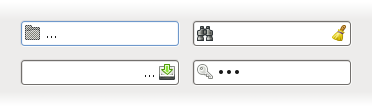
\includegraphics[width=75mm]{images/entry-icons.png}
\caption{Ikonok használata szövegbevteli mezőben}
\end{center}
\end{figure}

\paragraph{keresés} Egy-egy ikonnal jelezhetjük a beviteli mező két oldalán, hogy a beírt értéket keresni szeretnénk a valamely tartalomban -- legyen az egy több soros beviteli mező, egy fájl, vagy bármi más --, míg a másik ikon szolgálhat a keresési kifejezés törlésére.
\index{GtkEntry@\texttt{GtkEntry}!tulajdonságok!caps-lock-warning@\texttt{caps-lock-warning}}
\paragraph{jelszóbevitel} A jelszavak bevitelekor ikonnal jelezhetjük, hogy a megjelenő karakterek nem véletlenül nem az általunk beírtakat mutatják, a másik ikon pedig figyelmeztetésül szolgálhat, hogy ha a \textit{caps lock} be van kapcsolva\footnote{Ezt funkciót készen kapjuk a \texttt{GtkEntry} esetén, be-, illetve kikapcsolása a \texttt{caps-lock-warning} tulajdonság állításával lehetséges.}.
\paragraph{fájlműveletek} Fájlnevek bevitelekor jelezhetjük a felhasználó felé, hogy e mezőben szereplő fájlév mire szolgál majd voltaképp. Ezen túlmenően az ikonra kattintva felhozhatjuk a fájlválasztásra szolgáló dialógust.

\subsection{Folyamatindikátor}
\index{GtkEntry@\texttt{GtkEntry}!tulajdonságok!progress-pulse@\texttt{progress-pulse}}
\index{GtkEntry@\texttt{GtkEntry}!tulajdonságok!progress-pulse-step@\texttt{progress-pulse-step}}

A beviteli mező háttereként használhatunk folyamatindikátort, amivel jelezhetjük egy --  a beviteli mező tartalmával összefüggő -- folyamat állását. Amennyiben a folyamatot magát akarjuk érzékeltetni, viszont nem ismerjük annak végét, illetve aktuális állását, akkor választhatunk egy olyan módot ahol a folyamatindikátor a beviteli mező két vége között pulzál, ahol a \texttt{progress\_pulse} függvény hívásával mozdíthatjuk tovább a folyamatindikátort a \texttt{progress-pulse-step} tulajdonság által meghatározott (0 és egy közötti érték) mértékben.

\begin{figure}[h]
\begin{center}
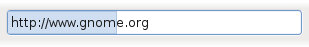
\includegraphics[width=75mm]{images/entry-with-progressbar.png}
\caption{Ikonok használata szövegbevteli mezőben}
\end{center}
\end{figure}

\index{GtkEntry@\texttt{GtkEntry}!tulajdonságok!progress-fraction@\texttt{progress-fraction}}
Amennyiben a folyamat állapota pontosan ismert, akkor az ábrához hasonló eredmény -- ahol az indikátor a folyamat állapotának mértékében foglalja el a hátteret --, a \texttt{progress-fraction} tulajdonság állításával érhető el, ahol az érték 0 és 1 között a folyamat készenléte.

\subsection{Iránymutató szöveg}

\index{GtkEntry@\texttt{GtkEntry}!tulajdonságok!placeholder-text@\texttt{placeholder-text}}
\index{GtkEntry@\texttt{GtkEntry}!függvények!set\_placeholder\_text@\texttt{set\_placeholder\_text}}
Egy beviteli mezők esetén -- legyen az szöveg vagy szám bevitelére szánva -- nincs kevésbé felhasználóbarát viselkedés, mint hogy a \textit{widget} semmilyen utalást nem tartalmaz arra nézvést, mit is kellene voltaképp tartalmazni. Erre természetesen alkalmas megoldás az előző részben megismert címke, illetve súgóbuborék, de a \texttt{GtkEntry}, valamint az abból származó \textit{widget}ek is rendelkeznek egy említésre érdemes megoldással. Ez pedig nem más, mint hogy a beviteli mezőbe egy olyan szöveget írhatunk, ami addig látszik, amíg  felhasználó a mezőbe írni nem kezd, vagy az írás végeztével üresen hagy. Ez a szöveg szolgálhat mintául a beírandó adat tartalmára, formájára és teszi ezt anélkül, hogy felhasználó interakciót igényelne, mint a súgóbuborék. Ezen szöveg a megadására az \texttt{GtkEntry} osztály \texttt{set\_paceholder\_text} függvénye szolgál.

\subsection{Buffer}
\index{GtkEntryBuffer@\texttt{GtkEntryBuffer}}

A \texttt{GtkEntry} típus esetén az adattároló réteg (model) elválasztásra került a megjelenítést, illetve vezérlést (view, controller) rétegtől, ami a tulajdonképpeni \texttt{GtkEntry}. Egy \texttt{GtkEntry} létrehozható paraméterek nélkül, vagy adattárolást végző típus -- a \texttt{GtkEntryBuffer} -- egy példányának megadásával. Ez egyrészt lehetővé teszi, hogy több, a megjelenítést végző \textit{widget}, osztozzon ugyanazon az adattárolón eltérő kijelölés, vagy éppen kurzorpozíció mellet. Másrészről leszármazva a \texttt{GtkEntryBuffer} buffer típusból, magunk is implementálhatunk adattárolót melyek a legkülönbözőbb igényeknek tehetnek eleget.

\subsection{Formázás}
\index{GtkSpinButton@\texttt{GtkSpinButton}}
\index{GtkSpinButton@\texttt{GtkSpinButton}!szignálok!input@\texttt{input}}
\index{GtkSpinButton@\texttt{GtkSpinButton}!szignálok!output@\texttt{output}}

A \texttt{GtkSpinButton} esetén magunk is meghatározhatjuk, hogy a tárolt adatot milyen formátumban fogadjuk el, illetve milyen formában jelenítjük meg. Ehhez nem kell egyebet tennünk, mint az \texttt{input}, illetve az \texttt{output} szignálokra megfelelő kezelő függvényeket kötni.

\lstdoublecsource
[language=C]
{sources/spin_button_input.c}
{sources/spin_button_output.c}
{Az \texttt{input} és \texttt{output} szignálok felüldefiniálása az alapértelmezett működést implementálva}
{lst:entryinputoutput}

\begin{description}
 \item[\ref{spinbuttonformatc:output}. sor] Az \texttt{input} és az \texttt{output} szignál kezelésére szolgáló függvény annyiban tér el egymástól amennyiben a feladat.

Az \texttt{input} szignált kezelő plusz paramétere (\texttt{new\_value}) -- az \texttt{input} kezelő függvényéhez képest --, a szövegként elérhető érték lebegőpontos számként történő visszaadására szolgál.
 \item[\ref{spinbuttonformatc:outputreturn}. sor] A visszatérési érték \texttt{TRUE} értéke mindkét esetben azt jelenti, hogy a szignált sikeresen kezeltük, az átalakítást elvégeztük. A \texttt{FALSE} visszatérési érték esetén a hívó az alapértelmezett átalakító függvényt -- aminek működése azonos a bemutatottal -- hívja meg.

Az \texttt{input} szignál esetén lehetséges még egy visszatérési érték (\texttt{GTK\_INPUT\_ERROR}), ami arra használunk, hogy a hívó felé jelezzük, a \texttt{GtkSpinButton} szövege nem értelmezhető. Ezért is \texttt{gint} ezen függvény visszatérési értékének típusa, míg a másiké \texttt{gboolean}, hisz ott csak azt közölhetjük a \texttt{GtkSpinButton} a beírást azt általunk kívánt formátumban megtettük-e vagy sem.
 \item[\ref{spinbuttonformatc:outputset}. sor] Az \texttt{input} esetén alapértelmezetten a \texttt{GtkSpinButton} szövegét decimális számrendszerbeli tizedes törtté próbáljuk alakítani. Ha ez sikerül \texttt{TRUE} értékkel térünk vissza, ha nem, akkor a visszatérési érték \texttt{GTK\_INPUT\_ERROR} jelezvén, hogy kezeltük az \texttt{input} szignált, de az átalakítás sikertelen volt, így az alapértelmezetten \texttt{input} szignált kezelő függvényt szükségtelen meghívni.

Az \texttt{output} szignál kezelésekor épp ez előbbiek ellenkezője történik. A \texttt{GtkSpinButton} aktuális számszerű értékét alakítjuk a megfelelő formátumú szöveggé. Ez esetben a \texttt{digits} tulajdonságnak megfelelő számú tizedes jeggyel decimális formában. Ezt írjuk vissza a beviteli mezőbe. A visszaírás viszont csak akkor történik meg, ha az a korábbi értéktől különbözik.
\end{description}

Az \texttt{input} és \texttt{output} szignálok felhasználására kézenfekvő példa lehet, hogy ha nem decimális számrendszerben szeretnénk a számokat megjeleníteni. Ez esetben a \texttt{g\_strtod} függvény helyett -- ami csak tízes számrendszerbeli számokkal működik -- a \texttt{g\_strtoull} függvény használható, ami a araméterként kapott számrendszerrel képes dolgozni, illetve a \texttt{g\_strdup\_printf} függvény esetén a formátum leírót kell a számrendszernek megfelelően módosítani (pl: \texttt{\%.*x} tizenhatos számrendszer esetén).

Ettől tágabban is értelmezhetjük a be-, illetve kimenet módosítását. Lehetőségünk van akár arra is, hogy a \texttt{GtkSpinButton} ne számokat tároljon, hanem szövegeket, például a hónapok neveit.

\lstdoublecsource
[language=C]
{sources/spin_button_input_hex.c}
{sources/spin_button_output_hex.c}
{Az \texttt{input} és \texttt{output} szignálok felüldefiniálása hónapok megjelenítéséhez}
{lst:entryinputoutputmonth}

Ebben az esetben nem történik más, mint hogy a formázást némiképp továbbgondoljuk. Az \texttt{input} szignál kezelésekor -- ahogy a korábbi példában is --, megpróbáljuk a beírt szöveget a formátumnak megfelelően értelmezni. Ez korábban annyit jelentett, hogy tizenhatos számrendszerbeli számként próbáltuk a szöveget értelmezni, most viszont -- mivel az értékkészletünk kicsi -- ellenőrizzük, hogy a beírt szöveg az értékkészlet (hónapok nevei) valamelyik eleme-e. Ha igen, akkor a hónap sorszáma lesz az új értékünk, ha nem akkor \texttt{GTK\_INPUT\_ERROR} értékkel térünk vissza.

A formázás -- vagyis az \texttt{output} szignál kezelése --, során mindössze az aktuális értéknek megfelelő szöveget kapja értékül a \texttt{GtkSpinButton}, feltéve ha eddig nem ez volt az értéke.

Természetesen egy ilyen formázási megoldásnál célszerű a \texttt{GtkSpinButton} minimum és maximum értékét az általunk kezelt értékek számosságának megfelelően beállítani, ami a hónapok esetén egyet jelent, mint minimum értéket és tizenkettőt, mint maximumot.

\section{Tesztelés}

Lévén a beviteli mezők a leggyakrabban használt \textit{widget}ek, tesztelésük is épp ily gyakran fordul elő. Ennek kapcsán megismerkedünk néhány -- a tesztelés során használt -- alapfogalommal, amik a későbbiekben is folyamatosan visszatérnek.

\subsection{Keresés}

Az ebben a részben tárgyalt két \textit{widget}típushoz -- az szöveg-, illetve számbeviteli mező -- tartozó objektumok keresésekor a \texttt{GenericPredicate} \texttt{roleName} paraméterének \texttt{text}, illetve \texttt{spin button} adandó meg. A \texttt{GtkEntry} kereséséhez létezik egy specializált \texttt{Predicate} osztály is, a \texttt{IsATextEntryNamed}, aminek egyetlen paramétere a beviteli mező neve.

\subsection{Interfészek}

\subsubsection{Írható szövegek}

Az adatbevitelre szolgáló \textit{widget}ekből értelemszerűen nem, vagy nem csak kiolvasni szeretnénk értéküket, de írni is, így ismerve a \textit{text} interfész adta lehetőségeket, ehhez egy másik mód lesz szükséges. Ez a mód egy külön interfész, amin a \textit{ATK} \texttt{EditableText} néven definiál és ami lehetővé teszi, hogy szövege írjunk, szúrjunk be, vagy illesszünk be a beviteli mezőbe. A legegyszerűbb esetben, amikor csak egy adott szöveggel szeretnénk felülírni a beviteli mező aktuális tartalmát erre az interfészre nem lesz szükségünk, a korábban a \textit{text} interfésznél ismertetett \texttt{text} attribútumnak való értékadás pontosan ezt teszi. Természetesen ennek megvan a megfelelője a \texttt{queryEditableText} függvényhívás révén beszerezhető \textit{editable text} interfészben is, mégpedig a \texttt{setTextContents} függvény, aminek paraméterül a beírandó szöveget kell átadnunk. Szöveg beszúrására is van lehetőség a \texttt{insertText} függvénnyel, aminek paraméterei a beszúrás pozíciója, a beszúrandó szöveg, illetve a beszúrandó karakterek száma.

A vágólap műveletek szintén ezen az interfészen keresztül érhetőek el. A másolás (\texttt{copyText}), törlés (\texttt{deleteText}), illetve kivágás (\texttt{cutText}) függvényinek két paramétert vesznek át, a szövegrész kezdő-, illetve végpozícióját amin a műveletet végre akarjuk hajtani. A beillesztés (\texttt{pasteText}) függvénynek csak egy paraméterre, a beillesztés helyére van szüksége.

\subsubsection{Számok}

Azon \textit{widget}típusokat, amiket számok bevitelére használunk nyilvánvalóan a tesztelés során is így szeretnénk kezelni, azzal együtt is, hogy voltaképpen szövegként szövegként is kiolvashatnánk, vagy beírhatnánk a bennük lévő adatot, és aztán a konverziót megejthetnénk magunk. Az \textit{ATK} szerencsénkre definiál a számok kezelésére használatos interfészt (\texttt{AtkValue}), így ezzel különösebb gondunk nem is lesz. Az interfész azonban nem csupán annyit nyújt, hogy számként írhatjuk, olvashatjuk az objektum tartalmát, de lehetőséget ad a mező által elfogadott intervallum alsó, illetve felső határának kiolvasására is. Az interfész lekérdezése a már megszokott elnevezési konvenció szerinti függvénnyel történik (\texttt{queryValue}), rajta keresztül az intervallum alsó határát a \texttt{minimumValue}, felső határát a \texttt{maximumValue}, míg aktuális értékét a \texttt{currentValue} attribútumon keresztül érhetjük el. Előbbi kettőt csak olvasásra, míg utóbbit írásra és olvasásra egyaránt. Gyakori esetről lévén szó ezen feladatok a \textit{Dogatil} \texttt{Node} osztályán keresztül is elvégezhetőek, rendre a \texttt{minValue}, \texttt{maxValue}, illetve a \texttt{value} attribútumok segítségével. Ez utóbbi megoldás előny, hogy megspórolhatjuk az interfész lekérdezését, illetve nem kell e kivételkezeléssel sem foglalkoznunk, mivel ha az interfész nem implementált, akkor lekérdezéskor a \texttt{NotImplementedError} kivétel helyett egyszerűen csak \texttt{None} értéket kapunk.

\subsection{Állapotok}

Mivel a beviteli mezőket tárgyaltunk ebben a részben, amik természetüknél fogva írhatóak, ugyanakkor lehetőség van arra a szerkeszthetőség letiltására, kézenfekvően adódik, hogy ezt az állapotot le is lehessen kérdezni. Ezt minden további nélkül meg is lehet tenni ha a már ismert \texttt{getState} függvénynek a \texttt{pyatspi.EDITABLE} értéket paraméterként. Egy másik állapot is kézenfekvően adódik a tárgyalt \textit{widget}ek típusából, mégpedig, hogy csak egy sornyi adat fogadására képesek, vagyis a \texttt{pyatspi.SINGLE\_LINE} állapot mindig része a \textit{widget} állapothalmazának, míg a \texttt{pyatspi.MULTI\_LINE} sosem.

\subsection{Tulajdonságok}

Mivel sem a \textit{text}, sem pedig az \textit{editable text} interfész nem ad módot rá módot, a már említett tulajdonságok (\texttt{attribute}) közül olvasható ki a \texttt{GtkEntry} osztály \texttt{set\_paceholder\_text} függvénye révén beállított szöveget, \texttt{placeholder-text} kulcs alatt.

\subsection{Akciók}

A gombokhoz hasonlóan a beviteli mezők is rendelkeznek egy rajtuk kiváltható akcióval, ez pedig a az alapértelmezett \textit{widget} aktiválása. Amennyiben a vonatkozó tulajdonság (\texttt{activates-default}) igaz, az \texttt{Node} objektumon -- a gombhoz hasonlóan végrehajtható -- az \texttt{activate} akció.
